\documentclass{ximera}

\graphicspath{{./content/02_4_curve_length/graphics/}{./graphics/}}

\title{The Length of a Curve}
\author{Melissa Lynn}
\outcome{Understand the definition and geometric significance of the length of a curve. Compute the lengths of parametric curves.}

\begin{document}
\begin{abstract}
\end{abstract}
\maketitle

We've defined paths and curves, and we've begun to study the behavior of paths through its velocity, speed, and acceleration. For curves, we would like to be able to quantify their inherent geometry, independent of their parametrization. That is, ignoring how we traverse a curve, how can we describe its shape?

We'll begin with a characteristic of a curve which should clearly be independent of parametrization: its length.

\section*{The Length of a Path}

Suppose we have a path $\vec{x}:I\rightarrow\mathbb{R}^n$, where $I$ is the interval $[a,b]$, and suppose we want to find the length of the corresponding curve $C$.

\begin{image}
\begin{tikzpicture}
\draw plot [thick, smooth, tension=.6] coordinates {(0,0) (1,1.312) (2, 1.5) (3,.937) (4,0) (5,-.937) (6, -1.5) (7, -1.312) (8,0)};
\filldraw (0,0) circle[radius=1pt];
\node[above left] at (0,0) {$\vec{x}(a)$};
\filldraw (8,0) circle[radius=1pt];
\node[above right] at (8,0) {$\vec{x}(b)$};
\end{tikzpicture}
\end{image}

We can approximate the curve with a lot of short line segments, and then compute the total length of the line segments to estimate the length of the curve.

\begin{image}
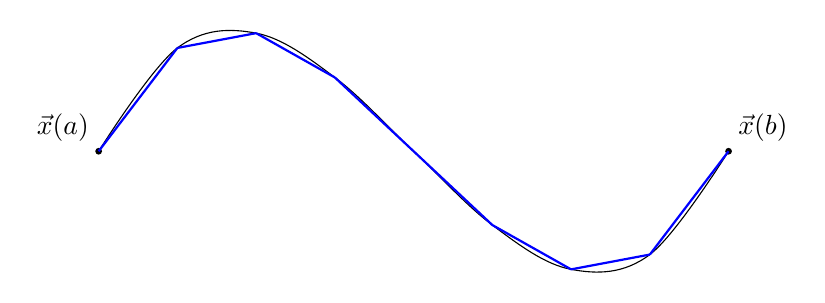
\begin{tikzpicture}
\draw plot [thick, smooth, tension=.6] coordinates {(0,0) (1,1.312) (2, 1.5) (3,.937) (4,0) (5,-.937) (6, -1.5) (7, -1.312) (8,0)};
\filldraw (0,0) circle[radius=1pt];
\node[above left] at (0,0) {$\vec{x}(a)$};
\filldraw (8,0) circle[radius=1pt];
\node[above right] at (8,0) {$\vec{x}(b)$};

\draw [thick, color = blue] (0,0) -- (1,1.312);
\draw [thick, color = blue] (1,1.312) -- (2,1.5);
\draw [thick, color = blue] (2,1.5) -- (3,.937);
\draw [thick, color = blue] (3,.937) -- (4,0);
\draw [thick, color = blue] (4,0) -- (5,-.937);
\draw [thick, color = blue] (5,-.937) -- (6,-1.5);
\draw [thick, color = blue] (6,-1.5) -- (7,-1.312);
\draw [thick, color = blue] (7,-1.312,0) -- (8,0);
\end{tikzpicture}
\end{image}


One way that we can do this is by subdividing the interval $[a,b]$ into $n$ subintervals $[t_{i-1},t_i]$ of equal length, and then take the line segments connecting $\vec{x}(t_{i-1})$ and $\vec{x}(t_i)$.

\begin{image}
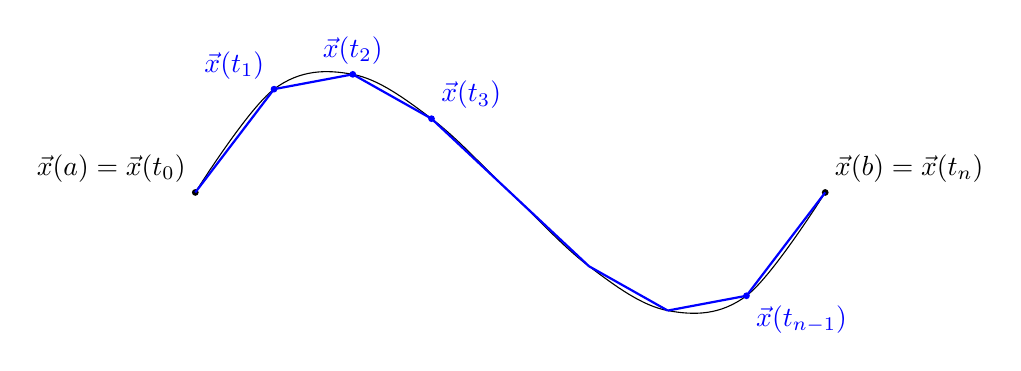
\begin{tikzpicture}
\draw plot [thick, smooth, tension=.6] coordinates {(0,0) (1,1.312) (2, 1.5) (3,.937) (4,0) (5,-.937) (6, -1.5) (7, -1.312) (8,0)};
\filldraw (0,0) circle[radius=1pt];
\node[above left] at (0,0) {$\vec{x}(a) = \vec{x}(t_0)$};
\filldraw (8,0) circle[radius=1pt];
\node[above right] at (8,0) {$\vec{x}(b) = \vec{x}(t_n)$};

\draw [thick, color = blue] (0,0) -- (1,1.312);
\filldraw [color = blue] (1,1.312) circle[radius=1pt];
\node[above left, color = blue] at (1,1.312) {$\vec{x}(t_1)$};
\draw [thick, color = blue] (1,1.312) -- (2,1.5);
\filldraw [color = blue] (2,1.5) circle[radius=1pt];
\node[above, color = blue] at (2,1.5) {$\vec{x}(t_2)$};
\draw [thick, color = blue] (2,1.5) -- (3,.937);
\filldraw [color = blue] (3,.937) circle[radius=1pt];
\node[above right, color = blue] at (3,.937) {$\vec{x}(t_3)$};
\draw [thick, color = blue] (3,.937) -- (4,0);
\draw [thick, color = blue] (4,0) -- (5,-.937);
\draw [thick, color = blue] (5,-.937) -- (6,-1.5);
\draw [thick, color = blue] (6,-1.5) -- (7,-1.312);
\filldraw [color = blue] (7,-1.312) circle[radius=1pt];
\node[below right, color = blue] at (7,-1.312) {$\vec{x}(t_{n-1})$};
\draw [thick, color = blue] (7,-1.312,0) -- (8,0);
\end{tikzpicture}
\end{image}

As $n$ increases, our line segments get shorter and shorter, giving us a more accurate approximation of the length of the curve. If $\vec{x}$ is a smooth parametrization of $C$, when we take the limit as $n\rightarrow\infty$, we will find the exact length of the curve.

Let's use this idea to find a formula for the length of a curve parametrized by a smooth path $\vec{x}(t)$. The length of the segment connecting $\vec{x}(t_{i-1})$ and $\vec{x}(t_i)$ can be computed as $\|\vec{x}(t_i)-\vec{x}(t_{i-1})\|$, so we have that the length of the curve is
\begin{align*}
L(\vec{x}) &\approx \sum_{i=1}^n\|\vec{x}(t_i)-\vec{x}(t_{i-1})\|\\
&=\sum_{i=1}^n\|\frac{\vec{x}(t_i)-\vec{x}(t_{i-1})}{\Delta t}\|\Delta t,
\end{align*}
where we both multiply and divide by $\Delta t$, the length of each subinterval.

As $n\rightarrow \infty$, the length of the subintervals, $\Delta t$, goes to $0$, and $\frac{\vec{x}(t_i)-\vec{x}(t_{i-1})}{\Delta t}$ goes to $\vec{x}'(t_i)$. This gives us
\[
L(\vec{x})=\lim_{n\rightarrow\infty}\sum_{i=1}^n \|\vec{x}'(t_i)\|\Delta.
\]
Recognizing this as an integral, we arrive at
\[
L(\vec{x}) = \int_a^b\|\vec{x}'(t)\|dt.
\]
Although we started with the goal of finding the length of a \emph{curve}, the result that we came up with could depend on the choice of parametrization $\vec{x}(t)$ of the curve. So, for now, we will use this idea to define the length of a path.

\begin{definition}
Let $\vec{x}:I\rightarrow\mathbb{R}^n$ be a $C^1$ path defined on the interval $I=[a,b]$. The \emph{length} of the path $\vec{x}$ is 
\[
L(\vec{x}) = \int_a^b\|\vec{x}'(t)\|dt.
\]
\end{definition} 

In the next section, we will explore how the choice of the parametrization affects the computation of the length of the corresponding curve. For now, we'll compute the length of paths in a couple of examples.

\begin{example}
Consider the path $\vec{x}:[0,2\pi]\rightarrow\mathbb{R}^2$ defined by $\vec{x}(t) = (\cos(t),\sin(t))$.

\begin{image}
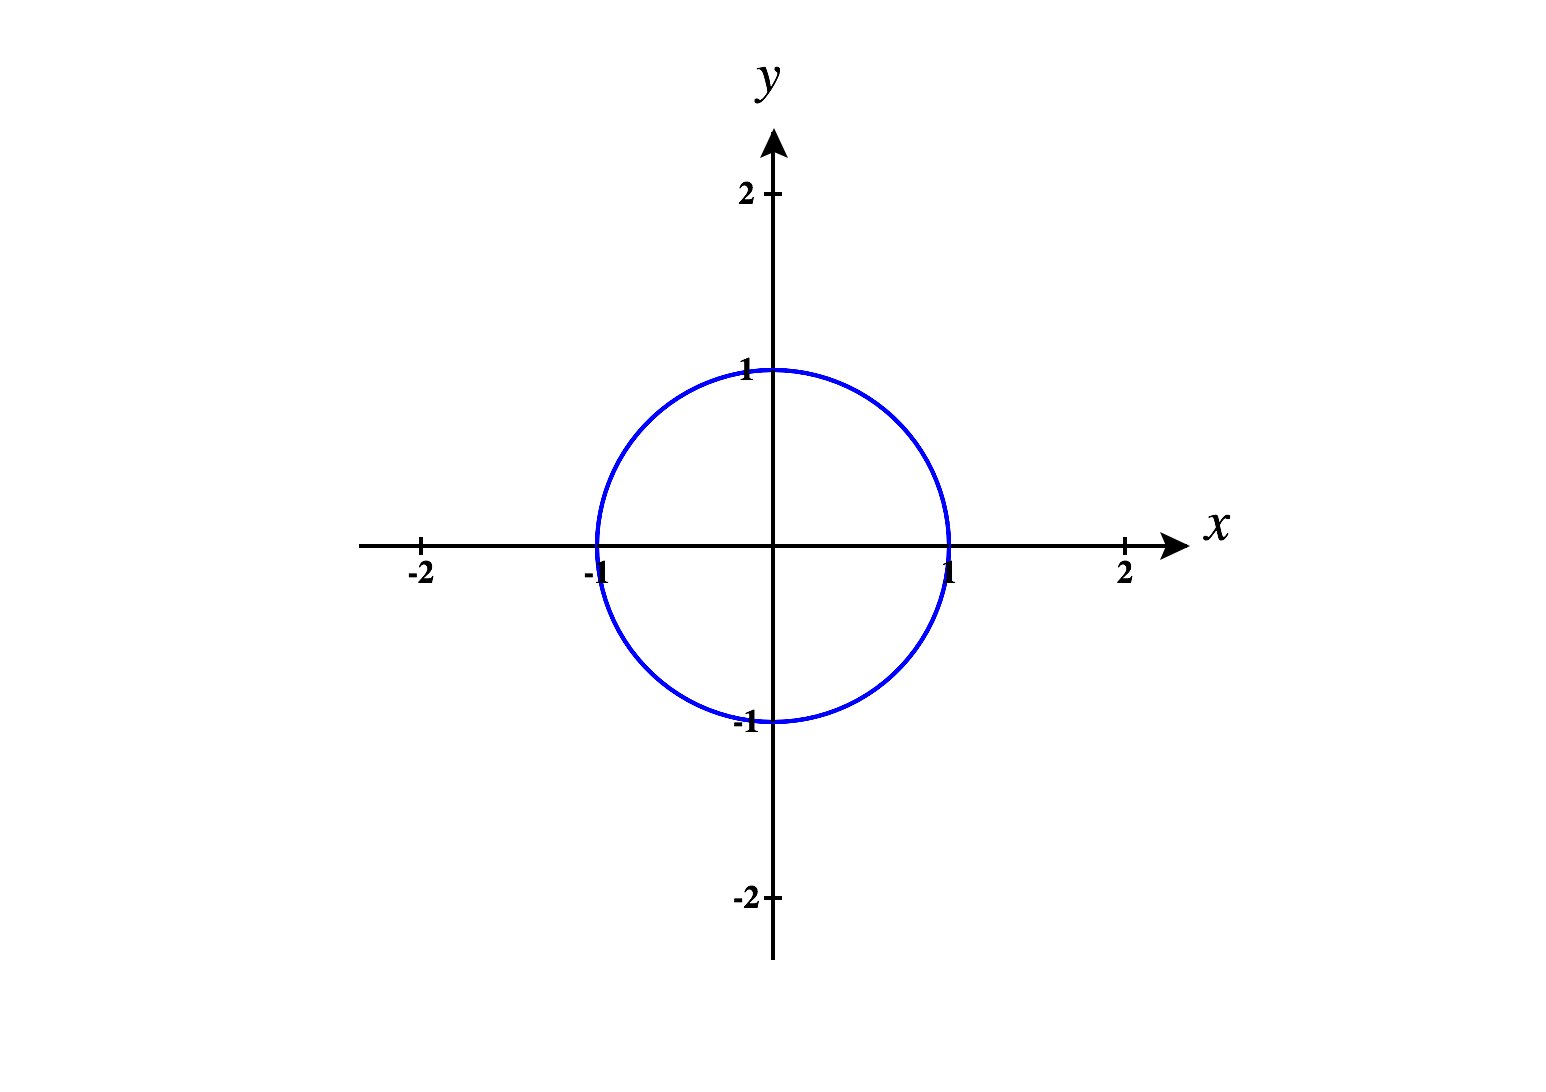
\includegraphics[width = \textwidth]{CalcPlot3D-unit_circle}
\end{image}

We compute the length of this path.
\begin{align*}
L(\vec{x}) &= \int_a^b\|\vec{x}'(t)\|dt\\
&= \int_{0}^{2\pi}\|(-\sin(t),\cos(t))\|dt\\
&= \int_{0}^{2\pi} \sqrt{(-\sin(t))^2 + (\cos(t))^2}\;dt\\
&= \int_{0}^{2\pi} \answer{1}dt\\
& = \answer{2\pi}
\end{align*}
Remembering that this is a parametrization for the unit circle, this matches with what we know to be the circumference of the circle.
\end{example}

\begin{example}
Consider the path $\vec{x}:[0,3\pi]\rightarrow\mathbb{R}^3$ defined by $\vec{x}(t) = (\cos(t),\sin(t),t)$.

\begin{image}
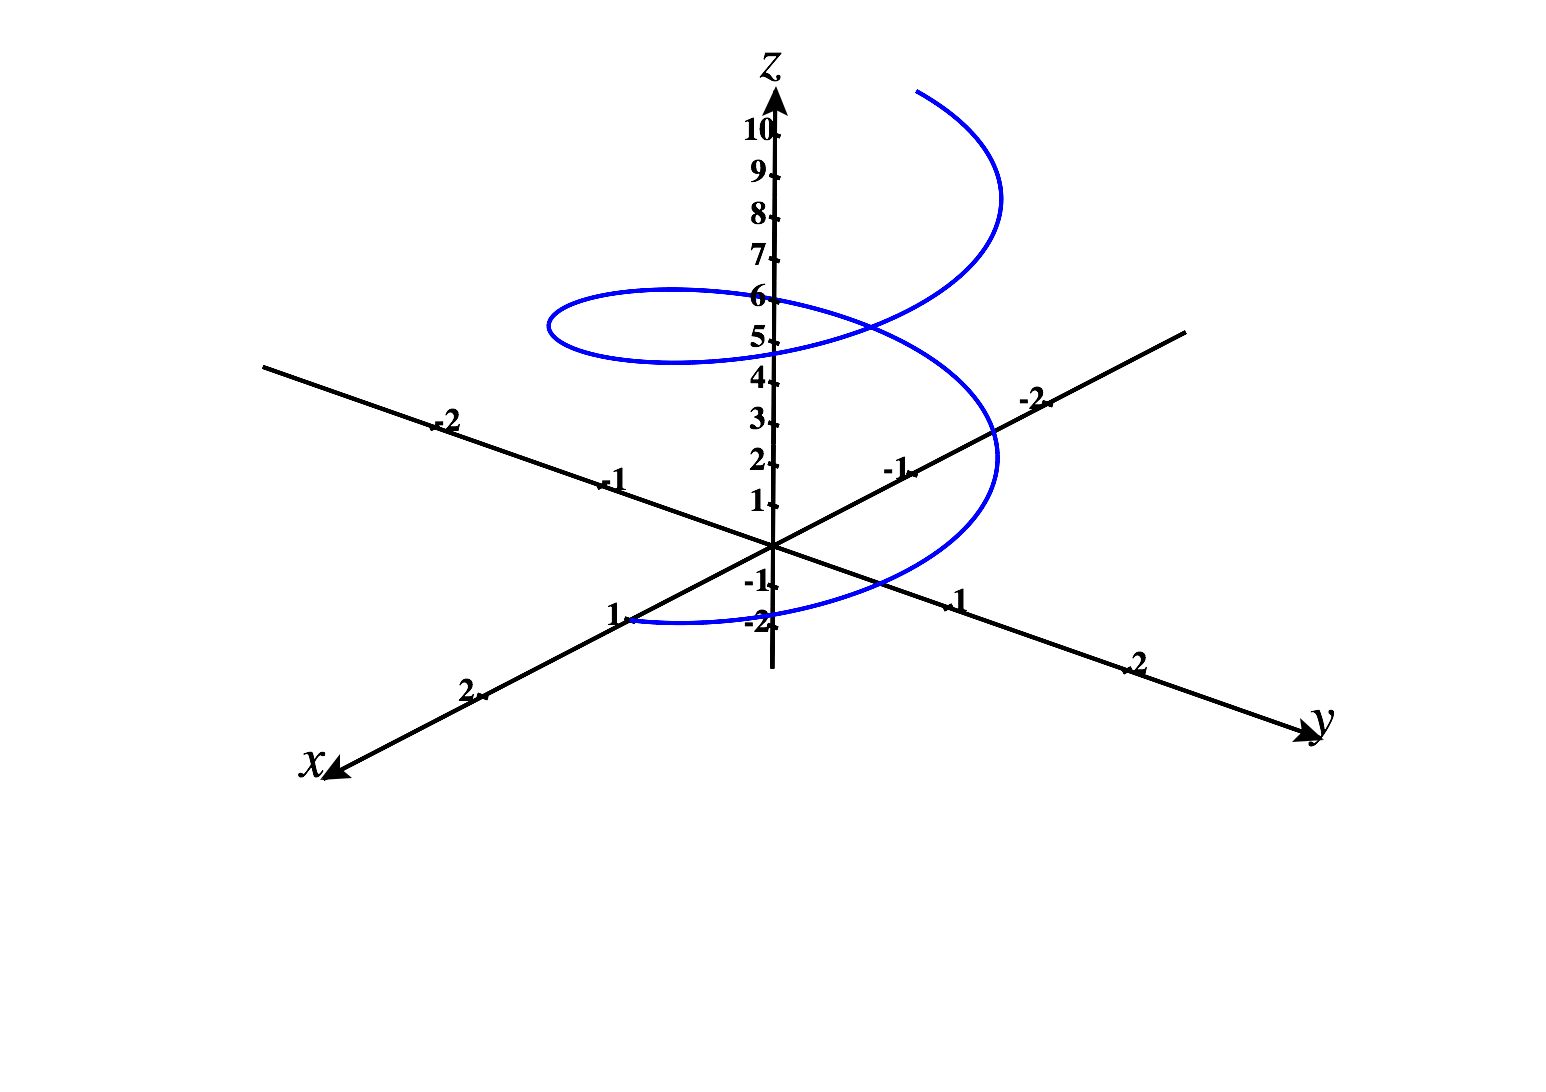
\includegraphics[width = \textwidth]{CalcPlot3D-spiral}
\end{image}

We compute the length of this path.
\begin{align*}
L(\vec{x}) &= \int_a^b\|\vec{x}'(t)\|dt\\
&= \int_{0}^{3\pi} \|\answer{(-\sin(t),\cos(t),1)}\|dt\\
&= \int_{0}^{3\pi} \answer{\sqrt{2}}dt\\
&= \answer{3\sqrt{2}\pi}
\end{align*}
\end{example}

Because of the square roots that appear when we take the magnitude of $\vec{x}'(t)$, arclength integrals for arbitrary curves are often messy to compute. However, in these cases, at least we can write down an integral representing the length of the curve, and perhaps use technology to either evaluate or approximate the integral.

\section*{The Length of a Curve}

In one of the previous examples, we found the length of the path $\vec{x}(t) = (\cos(t),\sin(t))$ for $t\in [0,2\pi]$. we found that $L(\vec{x}) = 2\pi$, matching what we know to be the circumference of the circle of radius $1$.

\begin{image}
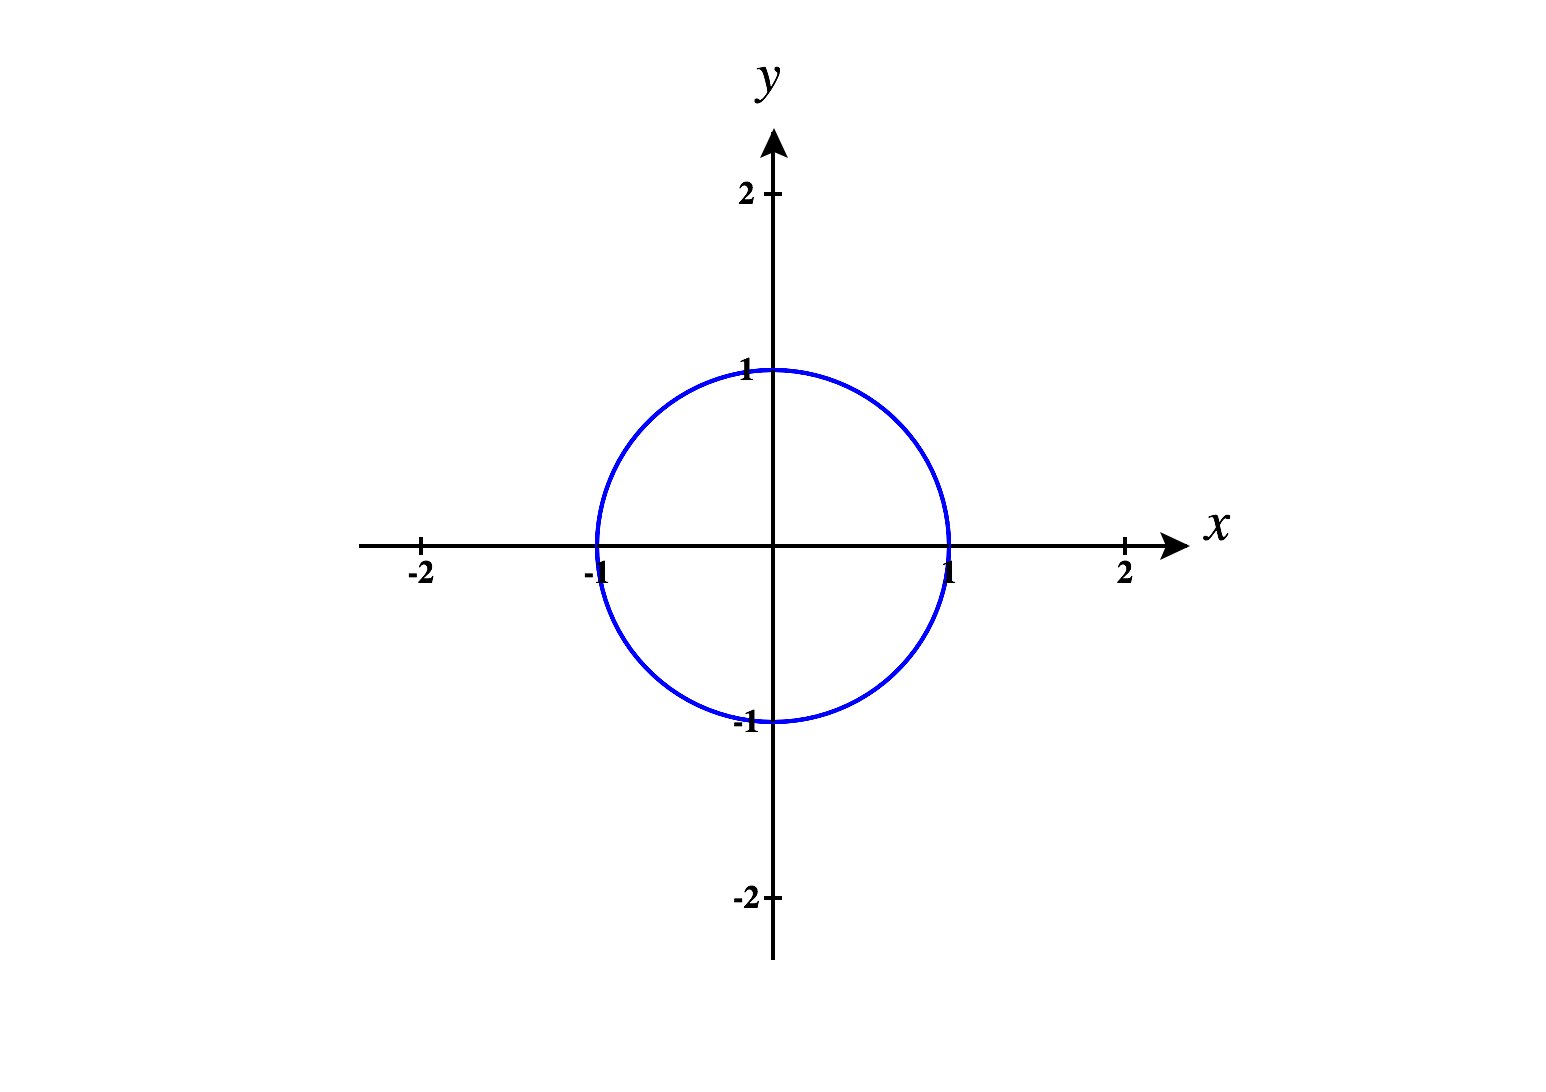
\includegraphics[width = \textwidth]{CalcPlot3D-unit_circle}
\end{image}

Let's see what happens when we take a different parametrization for the same curve, this time computing the length of $\vec{y}(t) = (\cos(t),\sin(t))$ for $t\in[0,4\pi]$. In this case, we get
\begin{align*}
L(\vec{x}) &= \int_a^b\|\vec{x}'(t)\|dt\\
&= \int_{0}^{4\pi}\|(-\sin(t),\cos(t))\|dt\\
&= \int_{0}^{4\pi} \sqrt{(-\sin(t))^2 + (\cos(t))^2}\;dt\\
&= \int_{0}^{4\pi} 1\;dt\\
& = \answer{4\pi}.
\end{align*}
Although $\vec{y}$ is another $C^1$ parametrization of the unit circle, we get a different result for the length of the path!

The issue here is that while $\vec{x}$ traces around the unit circle once, the path $\vec{y}$ traces around the unit circle twice. When we are computing $L(\vec{y})$, we are really computing the distance traced by the path $\vec{y}$, which is why we get twice the length of the actual curve.

Because of this, if we want to compute the length of a curve, we need to be careful with our choice of parametrization, to make sure that we are only tracing over the curve once. 

Fortunately, as long as we do not retrace our path, the length of a curve is independent of the parametrization. In order for this to be true, we require that a curve be \emph{simple}, which means that it does not intersect itself. More precisely, if $t_1\neq t_2$, then $\vec{x}(t_1)\neq \vec{x}(t_2)$.

The proof of the following theorem is left as an exercise. 

\begin{theorem}
Let $\vec{x}(t)$, for $a\leq t\leq b$, and $\vec{y}(s)$, for $c\leq s\leq d$, be smooth and simple parametrizations of the same curve $C$. Then $L(\vec{x}) = L(\vec{y})$.

In this case, we define the length of $C$ to be
\[
L(C) = L(\vec{x}) = L(\vec{y}).
\]
\end{theorem}

We also might encounter a situation where we want to compute the length of a curve which is not $C^1$, but is piecewise $C^1$. In this case, we can compute the length of the curve by computing the lengths of the pieces, and adding them together.

\begin{image}
\begin{tikzpicture}
\draw [thick] (0,0) -- (0,2) -- (4,2);
\draw plot [thick, smooth, tension=1] coordinates {(4,2) (6,0) (8,2)};
\filldraw (0,0) circle[radius=1pt];
\node[above left] at (0,0) {$\vec{x}(a)$};
\filldraw (8,2) circle[radius=1pt];
\node[above right] at (8,2) {$\vec{x}(b)$};
\end{tikzpicture}
\end{image}

\textit{Images were generated using \href{https://www.monroecc.edu/faculty/paulseeburger/calcnsf/CalcPlot3D/}{CalcPlot3D}.}

\end{document}